\documentclass[twoside]{book}

% Packages required by doxygen
\usepackage{fixltx2e}
\usepackage{calc}
\usepackage{doxygen}
\usepackage{graphicx}
\usepackage[utf8]{inputenc}
\usepackage{makeidx}
\usepackage{multicol}
\usepackage{multirow}
\PassOptionsToPackage{warn}{textcomp}
\usepackage{textcomp}
\usepackage[nointegrals]{wasysym}
\usepackage[table]{xcolor}

% Font selection
\usepackage[T1]{fontenc}
\usepackage{mathptmx}
\usepackage[scaled=.90]{helvet}
\usepackage{courier}
\usepackage{amssymb}
\usepackage{sectsty}
\renewcommand{\familydefault}{\sfdefault}
\allsectionsfont{%
  \fontseries{bc}\selectfont%
  \color{darkgray}%
}
\renewcommand{\DoxyLabelFont}{%
  \fontseries{bc}\selectfont%
  \color{darkgray}%
}
\newcommand{\+}{\discretionary{\mbox{\scriptsize$\hookleftarrow$}}{}{}}

% Page & text layout
\usepackage{geometry}
\geometry{%
  a4paper,%
  top=2.5cm,%
  bottom=2.5cm,%
  left=2.5cm,%
  right=2.5cm%
}
\tolerance=750
\hfuzz=15pt
\hbadness=750
\setlength{\emergencystretch}{15pt}
\setlength{\parindent}{0cm}
\setlength{\parskip}{0.2cm}
\makeatletter
\renewcommand{\paragraph}{%
  \@startsection{paragraph}{4}{0ex}{-1.0ex}{1.0ex}{%
    \normalfont\normalsize\bfseries\SS@parafont%
  }%
}
\renewcommand{\subparagraph}{%
  \@startsection{subparagraph}{5}{0ex}{-1.0ex}{1.0ex}{%
    \normalfont\normalsize\bfseries\SS@subparafont%
  }%
}
\makeatother

% Headers & footers
\usepackage{fancyhdr}
\pagestyle{fancyplain}
\fancyhead[LE]{\fancyplain{}{\bfseries\thepage}}
\fancyhead[CE]{\fancyplain{}{}}
\fancyhead[RE]{\fancyplain{}{\bfseries\leftmark}}
\fancyhead[LO]{\fancyplain{}{\bfseries\rightmark}}
\fancyhead[CO]{\fancyplain{}{}}
\fancyhead[RO]{\fancyplain{}{\bfseries\thepage}}
\fancyfoot[LE]{\fancyplain{}{}}
\fancyfoot[CE]{\fancyplain{}{}}
\fancyfoot[RE]{\fancyplain{}{\bfseries\scriptsize Generated on Sun Jan 15 2017 18\+:56\+:05 for Zumo Assignment by Doxygen }}
\fancyfoot[LO]{\fancyplain{}{\bfseries\scriptsize Generated on Sun Jan 15 2017 18\+:56\+:05 for Zumo Assignment by Doxygen }}
\fancyfoot[CO]{\fancyplain{}{}}
\fancyfoot[RO]{\fancyplain{}{}}
\renewcommand{\footrulewidth}{0.4pt}
\renewcommand{\chaptermark}[1]{%
  \markboth{#1}{}%
}
\renewcommand{\sectionmark}[1]{%
  \markright{\thesection\ #1}%
}

% Indices & bibliography
\usepackage{natbib}
\usepackage[titles]{tocloft}
\setcounter{tocdepth}{3}
\setcounter{secnumdepth}{5}
\makeindex

% Hyperlinks (required, but should be loaded last)
\usepackage{ifpdf}
\ifpdf
  \usepackage[pdftex,pagebackref=true]{hyperref}
\else
  \usepackage[ps2pdf,pagebackref=true]{hyperref}
\fi
\hypersetup{%
  colorlinks=true,%
  linkcolor=blue,%
  citecolor=blue,%
  unicode%
}

% Custom commands
\newcommand{\clearemptydoublepage}{%
  \newpage{\pagestyle{empty}\cleardoublepage}%
}


%===== C O N T E N T S =====

\begin{document}

% Titlepage & ToC
\hypersetup{pageanchor=false,
             bookmarks=true,
             bookmarksnumbered=true,
             pdfencoding=unicode
            }
\pagenumbering{roman}
\begin{titlepage}
\vspace*{7cm}
\begin{center}%
{\Large Zumo Assignment }\\
\vspace*{1cm}
{\large Generated by Doxygen 1.8.8}\\
\vspace*{0.5cm}
{\small Sun Jan 15 2017 18:56:05}\\
\end{center}
\end{titlepage}
\clearemptydoublepage
\tableofcontents
\clearemptydoublepage
\pagenumbering{arabic}
\hypersetup{pageanchor=true}

%--- Begin generated contents ---
\chapter{Main Page}
\label{index}\hypertarget{index}{}Zumo search and rescue robot using Arduino Uno.

Developed by Jack Allister (23042098)

\subsubsection*{Doxygen}

To access the doxygen output of the project please navigate to\+: {\itshape doxygen/html/index.\+html}

\section*{Functionality}


\begin{DoxyItemize}
\item Task 1 -\/ Wireless guided navigation.
\item Task 2 -\/ Path correction using reflectance sensors.
\item Task 3 -\/ Wall detection to stop the robot just before.
\item Task 4 -\/ Room search movement, allows the robot to move into a room for search.
\item Task 5 -\/ Uses the ultrasonic sensor to search a room for objects
\item Task 6 -\/ Robot can move autonomously to the begin, only searching rooms where objects were found.
\item Task 7 -\/ Not completed/implemented.
\end{DoxyItemize}

\subsection*{Wireless communication/movement.}

The robot is able to move wirelessly using the X\+Bee. This allows the robot to be controlled via simple terminally such as u\+Comm or Pu\+T\+T\+Y using the W\+A\+S\+D keys.

Important information is also sent from the robot back to the terminal such as found objects, movement etc.

\subsection*{Path correction}

Path correction is completed by using the reflectance sensors at the front-\/bottom of the robot.

The algorithm for detecting a wall is simple.

The robot checks every 50ms to see if a wall is detected on one of the outer reflectance sensors.

If so the robot stops it current motion, rotates away from the line and then continues it prior movement.

\subsection*{Wall detection}

Wall detection is implemented by checking the reflectance sensors as well.

If more than one reflectance sensor detects a wall/line boundary then the robot is stopped. This then allows the user to navigate the robot away from the wall (unless in autonomous mode).

\subsection*{Room Searching}

Room searching is implemented by using the ultrasonic sensors. At the moment a maximum range of 20cm from the robot is able to be searched, however this can be changed easily by changing one variable. Refer to check\+For\+Object procedure for more information.

\subsection*{Autonomous navigation}

Autonomous navigation is implemented by using a log of stored movements that are taken while in G\+U\+I\+D\+E\+D\+\_\+\+N\+A\+V\+I\+G\+A\+T\+E and S\+E\+A\+R\+C\+H\+\_\+\+R\+O\+O\+M mode. Wall sensing and path correction are both implemented within this mode so the robot should not be able to leave the specific boundaries of the course.

During the room searches in autonomous navigation, the robot will not search rooms that were found to be empty in user guided searching. This is a form of optimisation that would be crucial in a real world application of search and rescue.

\subsubsection*{Credits/\+References}


\begin{DoxyItemize}
\item New\+Ping library for ultrasonic sensor (Tim Eckel -\/ \href{mailto:teckel@leethost.com}{\tt teckel@leethost.\+com}) 
\end{DoxyItemize}
\chapter{Class Index}
\section{Class List}
Here are the classes, structs, unions and interfaces with brief descriptions\+:\begin{DoxyCompactList}
\item\contentsline{section}{\hyperlink{structMOVEMENT__COORD}{M\+O\+V\+E\+M\+E\+N\+T\+\_\+\+C\+O\+O\+R\+D} \\*Structure that is used for logging of actions }{\pageref{structMOVEMENT__COORD}}{}
\end{DoxyCompactList}

\chapter{File Index}
\section{File List}
Here is a list of all documented files with brief descriptions\+:\begin{DoxyCompactList}
\item\contentsline{section}{robotcode/\hyperlink{robotcode_8ino}{robotcode.\+ino} \\*Zumo Search and Rescue Robot using Arduino Uno }{\pageref{robotcode_8ino}}{}
\end{DoxyCompactList}

\chapter{Class Documentation}
\hypertarget{structMOVEMENT__COORD}{\section{M\+O\+V\+E\+M\+E\+N\+T\+\_\+\+C\+O\+O\+R\+D Struct Reference}
\label{structMOVEMENT__COORD}\index{M\+O\+V\+E\+M\+E\+N\+T\+\_\+\+C\+O\+O\+R\+D@{M\+O\+V\+E\+M\+E\+N\+T\+\_\+\+C\+O\+O\+R\+D}}
}


Structure that is used for logging of actions.  


\subsection*{Public Attributes}
\begin{DoxyCompactItemize}
\item 
\hypertarget{structMOVEMENT__COORD_a0c9331c535e2f29e15afd2a3f9b58da4}{\hyperlink{robotcode_8ino_a980e950615d86dadef54f3cfaefb5fb4}{O\+P\+E\+R\+A\+T\+I\+N\+G\+\_\+\+M\+O\+D\+E} {\bfseries mode}}\label{structMOVEMENT__COORD_a0c9331c535e2f29e15afd2a3f9b58da4}

\item 
\hypertarget{structMOVEMENT__COORD_a047c0f163ebf1b8d20961ca37aa4539a}{\hyperlink{robotcode_8ino_adc716dd21485bffb9015eaeb3cfe6859}{M\+O\+V\+E\+M\+E\+N\+T} {\bfseries movement}}\label{structMOVEMENT__COORD_a047c0f163ebf1b8d20961ca37aa4539a}

\item 
\hypertarget{structMOVEMENT__COORD_ad2bf7f74f2489fc76f8ba8590835d040}{unsigned long {\bfseries time}}\label{structMOVEMENT__COORD_ad2bf7f74f2489fc76f8ba8590835d040}

\item 
\hypertarget{structMOVEMENT__COORD_a7a052451926c762dfcc4df2c41e4a0b1}{int {\bfseries room\+I\+D}}\label{structMOVEMENT__COORD_a7a052451926c762dfcc4df2c41e4a0b1}

\end{DoxyCompactItemize}


\subsection{Detailed Description}
Structure that is used for logging of actions. 

Stores the current operating mode of the robot when logged.~\newline
Movement so that the movement can be replicated in autonomous.~\newline
The overall time that this action is taking place for.~\newline
The current room\+I\+D/number, if in a corridor stored as -\/1. 

The documentation for this struct was generated from the following file\+:\begin{DoxyCompactItemize}
\item 
robotcode/\hyperlink{robotcode_8ino}{robotcode.\+ino}\end{DoxyCompactItemize}

\chapter{File Documentation}
\hypertarget{robotcode_8ino}{\section{robotcode/robotcode.ino File Reference}
\label{robotcode_8ino}\index{robotcode/robotcode.\+ino@{robotcode/robotcode.\+ino}}
}


Zumo Search and Rescue Robot using Arduino Uno.  


{\ttfamily \#include $<$Zumo\+Motors.\+h$>$}\\*
{\ttfamily \#include $<$Q\+T\+R\+Sensors.\+h$>$}\\*
{\ttfamily \#include $<$Zumo\+Reflectance\+Sensor\+Array.\+h$>$}\\*
{\ttfamily \#include $<$New\+Ping.\+h$>$}\\*
Include dependency graph for robotcode.\+ino\+:\nopagebreak
\begin{figure}[H]
\begin{center}
\leavevmode
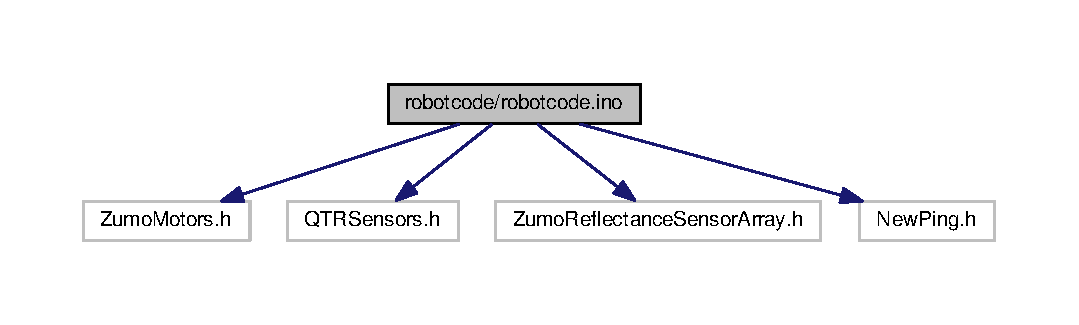
\includegraphics[width=350pt]{robotcode_8ino__incl}
\end{center}
\end{figure}
\subsection*{Classes}
\begin{DoxyCompactItemize}
\item 
struct \hyperlink{structMOVEMENT__COORD}{M\+O\+V\+E\+M\+E\+N\+T\+\_\+\+C\+O\+O\+R\+D}
\begin{DoxyCompactList}\small\item\em Structure that is used for logging of actions. \end{DoxyCompactList}\end{DoxyCompactItemize}
\subsection*{Macros}
\begin{DoxyCompactItemize}
\item 
\hypertarget{robotcode_8ino_ab4553be4db9860d940f81d7447173b2f}{\#define {\bfseries L\+E\+D\+\_\+\+P\+I\+N}~13}\label{robotcode_8ino_ab4553be4db9860d940f81d7447173b2f}

\item 
\hypertarget{robotcode_8ino_add02d1c189e3b727b722638327642a8b}{\#define {\bfseries N\+U\+M\+\_\+\+S\+E\+N\+S\+O\+R\+S}~6}\label{robotcode_8ino_add02d1c189e3b727b722638327642a8b}

\item 
\hypertarget{robotcode_8ino_adacee581176b7076b7baf0f72d81460f}{\#define {\bfseries T\+R\+I\+G\+G\+E\+R\+\_\+\+P\+I\+N}~2}\label{robotcode_8ino_adacee581176b7076b7baf0f72d81460f}

\item 
\hypertarget{robotcode_8ino_acea96cea4a13b6cb38e57a86788adf90}{\#define {\bfseries E\+C\+H\+O\+\_\+\+P\+I\+N}~3}\label{robotcode_8ino_acea96cea4a13b6cb38e57a86788adf90}

\item 
\hypertarget{robotcode_8ino_a08e4da5f3d0c7936fa52467f40e4b6aa}{\#define {\bfseries M\+A\+X\+\_\+\+D\+I\+S\+T\+A\+N\+C\+E}~20}\label{robotcode_8ino_a08e4da5f3d0c7936fa52467f40e4b6aa}

\item 
\hypertarget{robotcode_8ino_a8c43ff28382fa323973c476e7587b27f}{\#define {\bfseries M\+A\+X\+\_\+\+C\+O\+O\+R\+D\+I\+N\+A\+T\+E\+S}~60}\label{robotcode_8ino_a8c43ff28382fa323973c476e7587b27f}

\item 
\hypertarget{robotcode_8ino_a251d94cd24a2ca3369fc3f8eca8c19ae}{\#define {\bfseries M\+A\+X\+\_\+\+R\+O\+O\+M\+S}~5}\label{robotcode_8ino_a251d94cd24a2ca3369fc3f8eca8c19ae}

\item 
\hypertarget{robotcode_8ino_ac2cd96d53dd3ba6407db6766c3d92b26}{\#define {\bfseries M\+A\+X\+\_\+\+S\+P\+E\+E\+D}~120}\label{robotcode_8ino_ac2cd96d53dd3ba6407db6766c3d92b26}

\item 
\hypertarget{robotcode_8ino_acff0705eddd3534f7287eccf7bae20bb}{\#define {\bfseries C\+H\+A\+R\+\_\+\+C\+A\+L\+I\+B\+R\+A\+T\+E}~'1'}\label{robotcode_8ino_acff0705eddd3534f7287eccf7bae20bb}

\item 
\hypertarget{robotcode_8ino_a122a1d4695ae651ca004d41e1d00b6e4}{\#define {\bfseries C\+H\+A\+R\+\_\+\+C\+H\+E\+C\+K\+\_\+\+R\+O\+O\+M}~'2'}\label{robotcode_8ino_a122a1d4695ae651ca004d41e1d00b6e4}

\item 
\hypertarget{robotcode_8ino_a69a016ef92ad9ddb73560a123445502b}{\#define {\bfseries C\+H\+A\+R\+\_\+\+S\+T\+A\+R\+T\+\_\+\+A\+U\+T\+O\+N\+O\+M\+O\+U\+S}~'3'}\label{robotcode_8ino_a69a016ef92ad9ddb73560a123445502b}

\item 
\hypertarget{robotcode_8ino_a14691deb9ba5dc93a2bb3e0e8b4fdfd5}{\#define {\bfseries C\+H\+A\+R\+\_\+\+W\+A\+L\+L\+\_\+\+D\+E\+T\+E\+C\+T}~'C'}\label{robotcode_8ino_a14691deb9ba5dc93a2bb3e0e8b4fdfd5}

\item 
\hypertarget{robotcode_8ino_a663fe77d23ffb3b8c37f51583faf7c17}{\#define {\bfseries C\+H\+A\+R\+\_\+\+R\+O\+O\+M}~'R'}\label{robotcode_8ino_a663fe77d23ffb3b8c37f51583faf7c17}

\item 
\hypertarget{robotcode_8ino_a9a58b4c3522a04c4a0a65f9ad99f6a00}{\#define {\bfseries C\+H\+A\+R\+\_\+\+A\+U\+T\+O\+N\+O\+M\+O\+U\+S}~'E'}\label{robotcode_8ino_a9a58b4c3522a04c4a0a65f9ad99f6a00}

\item 
\hypertarget{robotcode_8ino_a764dbd349d8621accd792ee5210a3f74}{\#define {\bfseries C\+H\+A\+R\+\_\+\+F\+O\+R\+W\+A\+R\+D}~'W'}\label{robotcode_8ino_a764dbd349d8621accd792ee5210a3f74}

\item 
\hypertarget{robotcode_8ino_a1681b01a2698687a9b6aedd45b796f40}{\#define {\bfseries C\+H\+A\+R\+\_\+\+B\+A\+C\+K\+W\+A\+R\+D}~'S'}\label{robotcode_8ino_a1681b01a2698687a9b6aedd45b796f40}

\item 
\hypertarget{robotcode_8ino_aa05ecc497d01a93be5dd62ddaee54a75}{\#define {\bfseries C\+H\+A\+R\+\_\+\+L\+E\+F\+T}~'A'}\label{robotcode_8ino_aa05ecc497d01a93be5dd62ddaee54a75}

\item 
\hypertarget{robotcode_8ino_a94f7d75840f1acbd2c2acd01fc115d88}{\#define {\bfseries C\+H\+A\+R\+\_\+\+R\+I\+G\+H\+T}~'D'}\label{robotcode_8ino_a94f7d75840f1acbd2c2acd01fc115d88}

\item 
\hypertarget{robotcode_8ino_a245db460299318b2a2b61c2f884c1d19}{\#define {\bfseries C\+H\+A\+R\+\_\+\+S\+T\+O\+P}~0x20}\label{robotcode_8ino_a245db460299318b2a2b61c2f884c1d19}

\end{DoxyCompactItemize}
\subsection*{Enumerations}
\begin{DoxyCompactItemize}
\item 
enum \hyperlink{robotcode_8ino_a980e950615d86dadef54f3cfaefb5fb4}{O\+P\+E\+R\+A\+T\+I\+N\+G\+\_\+\+M\+O\+D\+E} \{ {\bfseries G\+U\+I\+D\+E\+D\+\_\+\+N\+A\+V\+I\+G\+A\+T\+E}, 
{\bfseries S\+E\+A\+R\+C\+H\+\_\+\+R\+O\+O\+M}, 
{\bfseries A\+U\+T\+O\+N\+O\+M\+O\+U\+S\+\_\+\+N\+A\+V\+I\+G\+A\+T\+E}
 \}
\begin{DoxyCompactList}\small\item\em enum for which operating 'mode' the robot is in \end{DoxyCompactList}\item 
enum \hyperlink{robotcode_8ino_adc716dd21485bffb9015eaeb3cfe6859}{M\+O\+V\+E\+M\+E\+N\+T} \{ \\*
{\bfseries F\+O\+R\+W\+A\+R\+D}, 
{\bfseries B\+A\+C\+K\+W\+A\+R\+D}, 
{\bfseries L\+E\+F\+T}, 
{\bfseries R\+I\+G\+H\+T}, 
\\*
{\bfseries S\+E\+A\+R\+C\+H}, 
{\bfseries N\+O\+N\+E}
 \}
\begin{DoxyCompactList}\small\item\em enum for which movement/action is taking place \end{DoxyCompactList}\end{DoxyCompactItemize}
\subsection*{Functions}
\begin{DoxyCompactItemize}
\item 
\hypertarget{robotcode_8ino_a9a97a20c8deb22c7db7d5cbd5d10a98f}{New\+Ping {\bfseries sonar} (T\+R\+I\+G\+G\+E\+R\+\_\+\+P\+I\+N, E\+C\+H\+O\+\_\+\+P\+I\+N, M\+A\+X\+\_\+\+D\+I\+S\+T\+A\+N\+C\+E)}\label{robotcode_8ino_a9a97a20c8deb22c7db7d5cbd5d10a98f}

\item 
void \hyperlink{robotcode_8ino_abbe89b02b936909feba8810c9675390f}{parse\+Guided\+Navigate} (char recv)
\begin{DoxyCompactList}\small\item\em Responsible for parsing special commands in G\+U\+I\+D\+E\+D\+\_\+\+N\+A\+V\+I\+G\+A\+T\+E mode. \end{DoxyCompactList}\item 
void \hyperlink{robotcode_8ino_aaaf5bee7c4545b94a6adda4907544241}{parse\+Search\+Room} (char recv)
\begin{DoxyCompactList}\small\item\em Responsible for parsing special commands in S\+E\+A\+R\+C\+H\+\_\+\+R\+O\+O\+M mode. \end{DoxyCompactList}\item 
bool \hyperlink{robotcode_8ino_adb00c91c925985a922f8c668dd439000}{parse\+Movement} (char recv)
\begin{DoxyCompactList}\small\item\em Responsible for parsing movement commands in any mode. \end{DoxyCompactList}\item 
void \hyperlink{robotcode_8ino_a28ad219170e626db83c63dfb8629d38c}{run\+Autonomous\+Mode} ()
\begin{DoxyCompactList}\small\item\em Runs the logged movements/actions stored from guided mode. \end{DoxyCompactList}\item 
\hyperlink{robotcode_8ino_adc716dd21485bffb9015eaeb3cfe6859}{M\+O\+V\+E\+M\+E\+N\+T} \hyperlink{robotcode_8ino_afe70bedfede401b2e61d7e2a54120bea}{calc\+Movement} (\hyperlink{structMOVEMENT__COORD}{M\+O\+V\+E\+M\+E\+N\+T\+\_\+\+C\+O\+O\+R\+D} mov)
\begin{DoxyCompactList}\small\item\em Calculates the optimised/needed movement needed in autonomos mode. \end{DoxyCompactList}\item 
void \hyperlink{robotcode_8ino_af776ff77e94170ec456760c6962020e5}{move\+Direction} (\hyperlink{robotcode_8ino_adc716dd21485bffb9015eaeb3cfe6859}{M\+O\+V\+E\+M\+E\+N\+T} movement)
\begin{DoxyCompactList}\small\item\em Moves the robot in a certain direction. \end{DoxyCompactList}\item 
bool \hyperlink{robotcode_8ino_ad8fb70ddbf7925148a848bd3c1df2b94}{check\+For\+Object} ()
\begin{DoxyCompactList}\small\item\em Uses the ultrasonic sensor to search the room for an object. \end{DoxyCompactList}\item 
bool \hyperlink{robotcode_8ino_abd77e61b6e1d72ce91e71cdbd86e3724}{correct\+Path} ()
\begin{DoxyCompactList}\small\item\em procedure for path correction to stop wall collisions \end{DoxyCompactList}\item 
bool \hyperlink{robotcode_8ino_a2d3a70671b195d39ddeb7a437b85d957}{is\+Wall\+Found} ()
\begin{DoxyCompactList}\small\item\em Checks to see if a wall is found using reflectance sensors. \end{DoxyCompactList}\item 
int \hyperlink{robotcode_8ino_a7a14e59caf883ee2936af076b102c68e}{is\+Sensors\+Over} (int start\+Sensor, int end\+Sensor)
\begin{DoxyCompactList}\small\item\em Function to check how many sensors are on a wall. \end{DoxyCompactList}\item 
void \hyperlink{robotcode_8ino_a11b381faabbecc0143d11cf09e955462}{calibrate\+Sensors} ()
\begin{DoxyCompactList}\small\item\em Calibrates the reflectance sensors on the robot. \end{DoxyCompactList}\item 
void \hyperlink{robotcode_8ino_a4fc01d736fe50cf5b977f755b675f11d}{setup} ()
\begin{DoxyCompactList}\small\item\em Runs once at boot of arduino. Responsible for settings up peripherals. \end{DoxyCompactList}\item 
void \hyperlink{robotcode_8ino_afe461d27b9c48d5921c00d521181f12f}{loop} ()
\begin{DoxyCompactList}\small\item\em System loop that is ran continuously. \end{DoxyCompactList}\item 
void \hyperlink{robotcode_8ino_a98da970f4d5707cef3faf45d97b2a0a9}{parse\+Autonomous} (char recv)
\begin{DoxyCompactList}\small\item\em Responsible for parsing special commands in A\+U\+T\+O\+N\+O\+M\+O\+U\+S\+\_\+\+N\+A\+V\+I\+G\+A\+T\+E mode. \end{DoxyCompactList}\end{DoxyCompactItemize}
\subsection*{Variables}
\begin{DoxyCompactItemize}
\item 
\hypertarget{robotcode_8ino_a107e8fa5802407f91589286783cb7c5d}{Zumo\+Motors {\bfseries motors}}\label{robotcode_8ino_a107e8fa5802407f91589286783cb7c5d}

\item 
\hypertarget{robotcode_8ino_a843402006805fb58c2fd952b79d491d8}{Zumo\+Reflectance\+Sensor\+Array {\bfseries reflectance\+Sensors}}\label{robotcode_8ino_a843402006805fb58c2fd952b79d491d8}

\item 
\hypertarget{robotcode_8ino_af589ed314ba3266f151b5c974f6868ea}{\hyperlink{robotcode_8ino_a980e950615d86dadef54f3cfaefb5fb4}{O\+P\+E\+R\+A\+T\+I\+N\+G\+\_\+\+M\+O\+D\+E} {\bfseries robot\+Mode} = G\+U\+I\+D\+E\+D\+\_\+\+N\+A\+V\+I\+G\+A\+T\+E}\label{robotcode_8ino_af589ed314ba3266f151b5c974f6868ea}

\item 
\hypertarget{robotcode_8ino_a834bdca1649fc7a14bcd0ef9c5d8b2ec}{\hyperlink{robotcode_8ino_adc716dd21485bffb9015eaeb3cfe6859}{M\+O\+V\+E\+M\+E\+N\+T} {\bfseries curr\+Movement} = N\+O\+N\+E}\label{robotcode_8ino_a834bdca1649fc7a14bcd0ef9c5d8b2ec}

\item 
\hypertarget{robotcode_8ino_a36454f4d674274472f062b8b609143a1}{bool {\bfseries wall\+Detect} = true}\label{robotcode_8ino_a36454f4d674274472f062b8b609143a1}

\item 
\hypertarget{robotcode_8ino_a90c3ccdd5d149c3fa002c1bb5bde0a20}{int {\bfseries room\+Count} = 0}\label{robotcode_8ino_a90c3ccdd5d149c3fa002c1bb5bde0a20}

\item 
\hypertarget{robotcode_8ino_a35b2ab6efdd73d9f5b5f60ea52b2fce2}{bool {\bfseries room\+Found} \mbox{[}M\+A\+X\+\_\+\+R\+O\+O\+M\+S\mbox{]} = \{false, false, false, false, false\}}\label{robotcode_8ino_a35b2ab6efdd73d9f5b5f60ea52b2fce2}

\item 
\hypertarget{robotcode_8ino_aa17773ebf8f2431cdae430c3aeb79fff}{\hyperlink{structMOVEMENT__COORD}{M\+O\+V\+E\+M\+E\+N\+T\+\_\+\+C\+O\+O\+R\+D} {\bfseries mov\+Log} \mbox{[}M\+A\+X\+\_\+\+C\+O\+O\+R\+D\+I\+N\+A\+T\+E\+S\mbox{]}}\label{robotcode_8ino_aa17773ebf8f2431cdae430c3aeb79fff}

\item 
\hypertarget{robotcode_8ino_a64310643aac4e3bb3b3a0c6117b3313b}{int {\bfseries mov\+Log\+Count} = 0}\label{robotcode_8ino_a64310643aac4e3bb3b3a0c6117b3313b}

\end{DoxyCompactItemize}


\subsection{Detailed Description}
Zumo Search and Rescue Robot using Arduino Uno. 

\begin{DoxyAuthor}{Author}
Jack Allister -\/ b3042098 
\end{DoxyAuthor}
\begin{DoxyDate}{Date}
15 Jan 2017 Implementation of the robot code for task 1-\/6 of assignment 1. Allows manual control, room searching and autonomous navigation. 
\end{DoxyDate}


\subsection{Enumeration Type Documentation}
\hypertarget{robotcode_8ino_adc716dd21485bffb9015eaeb3cfe6859}{\index{robotcode.\+ino@{robotcode.\+ino}!M\+O\+V\+E\+M\+E\+N\+T@{M\+O\+V\+E\+M\+E\+N\+T}}
\index{M\+O\+V\+E\+M\+E\+N\+T@{M\+O\+V\+E\+M\+E\+N\+T}!robotcode.\+ino@{robotcode.\+ino}}
\subsubsection[{M\+O\+V\+E\+M\+E\+N\+T}]{\setlength{\rightskip}{0pt plus 5cm}enum {\bf M\+O\+V\+E\+M\+E\+N\+T}}}\label{robotcode_8ino_adc716dd21485bffb9015eaeb3cfe6859}


enum for which movement/action is taking place 

Robot can be doing 1 of 6 possible movements at a time.~\newline
F\+O\+R\+W\+A\+R\+D, B\+A\+C\+K\+W\+A\+R\+D, L\+E\+F\+T, R\+I\+G\+H\+T~\newline
Searching or no action/movement. 
\begin{DoxyCode}
40 \{
41   FORWARD,
42   BACKWARD,
43   LEFT,
44   RIGHT,
45   SEARCH,
46   NONE
47 \} \hyperlink{robotcode_8ino_adc716dd21485bffb9015eaeb3cfe6859}{MOVEMENT};
\end{DoxyCode}
\hypertarget{robotcode_8ino_a980e950615d86dadef54f3cfaefb5fb4}{\index{robotcode.\+ino@{robotcode.\+ino}!O\+P\+E\+R\+A\+T\+I\+N\+G\+\_\+\+M\+O\+D\+E@{O\+P\+E\+R\+A\+T\+I\+N\+G\+\_\+\+M\+O\+D\+E}}
\index{O\+P\+E\+R\+A\+T\+I\+N\+G\+\_\+\+M\+O\+D\+E@{O\+P\+E\+R\+A\+T\+I\+N\+G\+\_\+\+M\+O\+D\+E}!robotcode.\+ino@{robotcode.\+ino}}
\subsubsection[{O\+P\+E\+R\+A\+T\+I\+N\+G\+\_\+\+M\+O\+D\+E}]{\setlength{\rightskip}{0pt plus 5cm}enum {\bf O\+P\+E\+R\+A\+T\+I\+N\+G\+\_\+\+M\+O\+D\+E}}}\label{robotcode_8ino_a980e950615d86dadef54f3cfaefb5fb4}


enum for which operating 'mode' the robot is in 

Robot can only be in one mode at a time.~\newline
G\+U\+I\+D\+E\+D\+\_\+\+N\+A\+V\+I\+G\+A\+T\+E -\/ Robot controlled wirelessly from a computer via X\+Bee.~\newline
S\+E\+A\+R\+C\+H\+\_\+\+R\+O\+O\+M -\/ Mode for searching a room, allows use of ultrasonic sensor.~\newline
A\+U\+T\+O\+N\+O\+M\+O\+U\+S\+\_\+\+N\+A\+V\+I\+G\+A\+T\+E -\/ Mode uses stored movements and actions to return to start.~\newline

\begin{DoxyCode}
26 \{
27   GUIDED\_NAVIGATE,
28   SEARCH\_ROOM,
29   AUTONOMOUS\_NAVIGATE
30 \} \hyperlink{robotcode_8ino_a980e950615d86dadef54f3cfaefb5fb4}{OPERATING\_MODE};
\end{DoxyCode}


\subsection{Function Documentation}
\hypertarget{robotcode_8ino_afe70bedfede401b2e61d7e2a54120bea}{\index{robotcode.\+ino@{robotcode.\+ino}!calc\+Movement@{calc\+Movement}}
\index{calc\+Movement@{calc\+Movement}!robotcode.\+ino@{robotcode.\+ino}}
\subsubsection[{calc\+Movement}]{\setlength{\rightskip}{0pt plus 5cm}{\bf M\+O\+V\+E\+M\+E\+N\+T} calc\+Movement (
\begin{DoxyParamCaption}
\item[{{\bf M\+O\+V\+E\+M\+E\+N\+T\+\_\+\+C\+O\+O\+R\+D}}]{mov}
\end{DoxyParamCaption}
)}}\label{robotcode_8ino_afe70bedfede401b2e61d7e2a54120bea}


Calculates the optimised/needed movement needed in autonomos mode. 

The optimised/needed movement is calculated using a switch case.~\newline
Because movements are parsed in a reverse order in run\+Autonomous\+Mode we needed to inverse some commands for example movements/actions taken place in S\+E\+A\+R\+C\+H\+\_\+\+R\+O\+O\+M mode.


\begin{DoxyParams}{Parameters}
{\em mov} & -\/ \hyperlink{structMOVEMENT__COORD}{M\+O\+V\+E\+M\+E\+N\+T\+\_\+\+C\+O\+O\+R\+D} structure/object from mov\+Log to be used in calculation. \\
\hline
\end{DoxyParams}
\begin{DoxyReturn}{Returns}
M\+O\+V\+E\+M\+E\+N\+T -\/ the optimised movement for the robot to take. 
\end{DoxyReturn}

\begin{DoxyCode}
484 \{
485   \hyperlink{robotcode_8ino_adc716dd21485bffb9015eaeb3cfe6859}{MOVEMENT} result = NONE;
486 
487   \textcolor{keywordflow}{switch} (mov.movement)
488   \{
489     \textcolor{keywordflow}{case} FORWARD:
490     \{
491       \textcolor{keywordflow}{if} (mov.mode == SEARCH\_ROOM)
492         result = BACKWARD;
493       \textcolor{keywordflow}{else}
494         result = FORWARD;
495       \textcolor{keywordflow}{break};
496     \}
497 
498     \textcolor{keywordflow}{case} BACKWARD:
499     \{
500       \textcolor{keywordflow}{if} (mov.mode == SEARCH\_ROOM)
501         result = FORWARD;
502       \textcolor{keywordflow}{else}
503         result = BACKWARD;
504       \textcolor{keywordflow}{break};
505     \}
506 
507     \textcolor{keywordflow}{case} LEFT:
508     \{
509       \textcolor{keywordflow}{if} (mov.mode == SEARCH\_ROOM)
510         result = LEFT;
511       \textcolor{keywordflow}{else}
512         result = RIGHT;
513       \textcolor{keywordflow}{break};
514     \}
515 
516     \textcolor{keywordflow}{case} RIGHT:
517     \{
518       \textcolor{keywordflow}{if} (mov.mode == SEARCH\_ROOM)
519         result = RIGHT;
520       \textcolor{keywordflow}{else}
521         result = LEFT;
522       \textcolor{keywordflow}{break};
523     \}
524   \}
525 
526   \textcolor{keywordflow}{return} result;
527 \}
\end{DoxyCode}
\hypertarget{robotcode_8ino_a11b381faabbecc0143d11cf09e955462}{\index{robotcode.\+ino@{robotcode.\+ino}!calibrate\+Sensors@{calibrate\+Sensors}}
\index{calibrate\+Sensors@{calibrate\+Sensors}!robotcode.\+ino@{robotcode.\+ino}}
\subsubsection[{calibrate\+Sensors}]{\setlength{\rightskip}{0pt plus 5cm}void calibrate\+Sensors (
\begin{DoxyParamCaption}
{}
\end{DoxyParamCaption}
)}}\label{robotcode_8ino_a11b381faabbecc0143d11cf09e955462}


Calibrates the reflectance sensors on the robot. 

Procedure calibrates the reflectance sensors by moving the robot backwards and forwards over a wall boundary.~\newline
This allows accurate wall detection. 
\begin{DoxyCode}
840 \{
841   \textcolor{keyword}{static} \textcolor{keyword}{const} \textcolor{keywordtype}{unsigned} \textcolor{keywordtype}{long} MOVE\_TIME = 350;
842 
843   \textcolor{keywordtype}{char} dummy;
844   \textcolor{keywordtype}{int} i;
845 
846   Serial.println(\textcolor{stringliteral}{"Calibrating sensors"});
847   Serial.println(\textcolor{stringliteral}{"Move the robot so that the sensors are just before a line/wall"});
848   Serial.println(\textcolor{stringliteral}{"Press space to continue"});
849   \textcolor{keywordflow}{while} (Serial.available() == 0)
850   \{
851 
852   \}
853   dummy = Serial.read();
854 
855   \textcolor{keywordflow}{for} (i = 0; i < 10; i++)
856   \{
857     \textcolor{keywordtype}{unsigned} \textcolor{keywordtype}{long} startTime = millis();
858     motors.setSpeeds(MAX\_SPEED, MAX\_SPEED);
859     \textcolor{keywordflow}{while} (millis() - startTime < MOVE\_TIME)
860     \{
861       reflectanceSensors.calibrate();
862     \}
863 
864     startTime = millis();
865     motors.setSpeeds(-MAX\_SPEED, -MAX\_SPEED);
866     \textcolor{keywordflow}{while} (millis() - startTime < MOVE\_TIME)
867     \{
868       reflectanceSensors.calibrate();
869     \}
870   \}
871   motors.setSpeeds(0, 0);
872 
873   \textcolor{keywordflow}{for} (i = 0; i < NUM\_SENSORS; i++)
874   \{
875     Serial.print(\textcolor{stringliteral}{"Minimum values: "});
876     Serial.print(reflectanceSensors.calibratedMinimumOn[i]);
877     Serial.print(\textcolor{charliteral}{' '});
878   \}
879   Serial.println();
880 
881   \textcolor{keywordflow}{for} (i = 0; i < NUM\_SENSORS; i++)
882   \{
883     Serial.print(\textcolor{stringliteral}{"Maximum values: "});
884     Serial.print(reflectanceSensors.calibratedMaximumOn[i]);
885     Serial.print(\textcolor{charliteral}{' '});
886   \}
887   Serial.println();
888 
889   Serial.println(\textcolor{stringliteral}{"Sensor calibration complete!"});
890 \}
\end{DoxyCode}
\hypertarget{robotcode_8ino_ad8fb70ddbf7925148a848bd3c1df2b94}{\index{robotcode.\+ino@{robotcode.\+ino}!check\+For\+Object@{check\+For\+Object}}
\index{check\+For\+Object@{check\+For\+Object}!robotcode.\+ino@{robotcode.\+ino}}
\subsubsection[{check\+For\+Object}]{\setlength{\rightskip}{0pt plus 5cm}bool check\+For\+Object (
\begin{DoxyParamCaption}
{}
\end{DoxyParamCaption}
)}}\label{robotcode_8ino_ad8fb70ddbf7925148a848bd3c1df2b94}


Uses the ultrasonic sensor to search the room for an object. 

Robot rotates left while the ultrasonic sensor is on to try and find objects. The robot then returns right while doing the same thing. Maximum distance for the ultrasonic sensor is set at 20cm using the constant M\+A\+X\+\_\+\+D\+I\+S\+T\+A\+N\+C\+E this can be changed to allow up to a maximum of 200cm.

\begin{DoxyReturn}{Returns}
boolean -\/ Whether an object was discovered. 
\end{DoxyReturn}

\begin{DoxyCode}
635 \{
636   \textcolor{keyword}{static} \textcolor{keyword}{const} \textcolor{keywordtype}{unsigned} \textcolor{keywordtype}{long} TURN\_TIME = 750;
637 
638   \textcolor{keywordtype}{bool} found = \textcolor{keyword}{false};
639   \textcolor{keywordtype}{unsigned} \textcolor{keywordtype}{long} startTime;
640   \textcolor{keywordtype}{unsigned} \textcolor{keywordtype}{long} pingDist;
641 
642   Serial.println(\textcolor{stringliteral}{"Checking room for objects"});
643   \textcolor{comment}{/* Perform a quick scan of the room using US to find items */}
644 
645   \textcolor{comment}{/* Check left direction */}
646   Serial.println(\textcolor{stringliteral}{"Checking left"});
647   motors.setSpeeds(-MAX\_SPEED, MAX\_SPEED);
648   startTime = millis();
649   \textcolor{keywordflow}{while} ((millis() - startTime) < TURN\_TIME)
650   \{
651     delay(50);
652     pingDist = sonar.ping\_cm();
653     \textcolor{keywordflow}{if} ((pingDist != 0) && (found == \textcolor{keyword}{false}))
654     \{
655       \textcolor{comment}{/* If we get here means object found in left of room */}
656       Serial.print(\textcolor{stringliteral}{"Object found in left of room "});
657       Serial.print(pingDist);
658       Serial.println(\textcolor{stringliteral}{" cm away."});
659       found = \textcolor{keyword}{true};
660     \}
661   \}
662 
663   \textcolor{comment}{/* Move right to midpoint */}
664   motors.setSpeeds(MAX\_SPEED, -MAX\_SPEED);
665   startTime = millis();
666   \textcolor{keywordflow}{while} ((millis() - startTime) < TURN\_TIME)
667   \{
668     \textcolor{comment}{/* Do nothing here as returning */}
669   \}
670 
671   \textcolor{comment}{/* Check right direction */}
672   Serial.println(\textcolor{stringliteral}{"Checking right"});
673   startTime = millis();
674   \textcolor{keywordflow}{while} ((millis() - startTime) < TURN\_TIME)
675   \{
676     delay(50);
677     pingDist = sonar.ping\_cm();
678     \textcolor{keywordflow}{if} ((pingDist != 0) && (found == \textcolor{keyword}{false}))
679     \{
680       \textcolor{comment}{/* If we get here means object found in right of room */}
681       Serial.print(\textcolor{stringliteral}{"Object found in right of room "});
682       Serial.print(pingDist);
683       Serial.println(\textcolor{stringliteral}{" cm away."});
684       found = \textcolor{keyword}{true};
685     \}
686   \}
687 
688   \textcolor{comment}{/* Move left to midpoint */}
689   motors.setSpeeds(-MAX\_SPEED, MAX\_SPEED);
690   startTime = millis();
691   \textcolor{keywordflow}{while} ((millis() - startTime) < TURN\_TIME)
692   \{
693     \textcolor{comment}{/* Do nothing here as returning */}
694   \}
695 
696   motors.setSpeeds(0, 0);
697   \textcolor{keywordflow}{if} (found == \textcolor{keyword}{false})
698     Serial.println(\textcolor{stringliteral}{"No objects found."});
699 
700   \textcolor{comment}{/* Method for storing movement coordinates */}
701   \textcolor{keywordflow}{if} (robotMode != AUTONOMOUS\_NAVIGATE)
702   \{
703     \textcolor{comment}{/* Set movement and start time */}
704     \textcolor{keywordtype}{unsigned} \textcolor{keywordtype}{long} currTime = millis();
705     movLog[movLogCount].mode = robotMode;
706     movLog[movLogCount].movement = SEARCH;
707     movLog[movLogCount].time = currTime;
708     movLog[movLogCount].roomID = roomCount;
709 
710     \textcolor{comment}{/* Here we correct previous log time so that it is delta/diff */}
711     \textcolor{keywordflow}{if} (movLogCount != 0)
712     \{
713       movLog[movLogCount-1].time = currTime - movLog[movLogCount-1].time;
714     \}
715     movLogCount++;
716   \}
717 
718   roomFound[roomCount] = found;
719   \textcolor{keywordflow}{return} found;
720 \}
\end{DoxyCode}
\hypertarget{robotcode_8ino_abd77e61b6e1d72ce91e71cdbd86e3724}{\index{robotcode.\+ino@{robotcode.\+ino}!correct\+Path@{correct\+Path}}
\index{correct\+Path@{correct\+Path}!robotcode.\+ino@{robotcode.\+ino}}
\subsubsection[{correct\+Path}]{\setlength{\rightskip}{0pt plus 5cm}bool correct\+Path (
\begin{DoxyParamCaption}
{}
\end{DoxyParamCaption}
)}}\label{robotcode_8ino_abd77e61b6e1d72ce91e71cdbd86e3724}


procedure for path correction to stop wall collisions 

Path correction that stops either the left or right side of the robot from accidentally driving over a wall boundary. This function uses the reflectance sensors to do so.~\newline
Path correction can only happen once every 50ms.

\begin{DoxyReturn}{Returns}
boolean -\/ Whether path correction has taken place. 
\end{DoxyReturn}

\begin{DoxyCode}
733 \{
734   \textcolor{keyword}{static} \textcolor{keyword}{const} \textcolor{keywordtype}{unsigned} \textcolor{keywordtype}{long} CORR\_INTERVAL = 50;
735   \textcolor{keyword}{static} \textcolor{keyword}{const} \textcolor{keywordtype}{int} LEFT\_START = 0;
736   \textcolor{keyword}{static} \textcolor{keyword}{const} \textcolor{keywordtype}{int} RIGHT\_START = 5;
737 
738   \textcolor{keyword}{static} \textcolor{keywordtype}{unsigned} \textcolor{keywordtype}{long} lastRun = 0;
739   \textcolor{keywordtype}{bool} result = \textcolor{keyword}{false};
740   \hyperlink{robotcode_8ino_adc716dd21485bffb9015eaeb3cfe6859}{MOVEMENT} lastMovement;
741 
742   \textcolor{comment}{/* Corrects the path to stop a side from accidentally going on a wall */}
743 
744   \textcolor{comment}{/* Correction happens every 50ms */}
745   \textcolor{keywordflow}{if} ((lastRun == 0) || (millis() - lastRun > CORR\_INTERVAL))
746   \{
747     lastRun = millis();
748 
749     \textcolor{comment}{/* Check to make sure only left sensor is on a line */}
750     \textcolor{keywordflow}{if} ((\hyperlink{robotcode_8ino_a7a14e59caf883ee2936af076b102c68e}{isSensorsOver}(LEFT\_START, LEFT\_START) > 0) &&
751         (\hyperlink{robotcode_8ino_a7a14e59caf883ee2936af076b102c68e}{isSensorsOver}(RIGHT\_START, RIGHT\_START) == 0))
752     \{
753       \textcolor{comment}{/* If true correct path by moving the robot right until not on line */}
754       motors.setSpeeds(MAX\_SPEED, -MAX\_SPEED);
755       \textcolor{keywordflow}{do}
756       \{
757 
758       \} \textcolor{keywordflow}{while} (\hyperlink{robotcode_8ino_a7a14e59caf883ee2936af076b102c68e}{isSensorsOver}(LEFT\_START, LEFT\_START) > 0);
759       motors.setSpeeds(MAX\_SPEED, MAX\_SPEED);
760 
761       Serial.println(\textcolor{stringliteral}{"Corrected left"});
762       result = \textcolor{keyword}{true};
763     \}
764     \textcolor{keywordflow}{else} \textcolor{keywordflow}{if} ((\hyperlink{robotcode_8ino_a7a14e59caf883ee2936af076b102c68e}{isSensorsOver}(RIGHT\_START, RIGHT\_START) > 0) &&
765              (\hyperlink{robotcode_8ino_a7a14e59caf883ee2936af076b102c68e}{isSensorsOver}(LEFT\_START, LEFT\_START) == 0))
766     \{
767       \textcolor{comment}{/* If true correct path by moving the robot left until not on line */}
768       motors.setSpeeds(-MAX\_SPEED, MAX\_SPEED);
769       \textcolor{keywordflow}{do}
770       \{
771 
772       \} \textcolor{keywordflow}{while} (\hyperlink{robotcode_8ino_a7a14e59caf883ee2936af076b102c68e}{isSensorsOver}(RIGHT\_START, RIGHT\_START) > 0);
773       motors.setSpeeds(MAX\_SPEED, MAX\_SPEED);
774 
775       \textcolor{comment}{/* If far right sensor on a line correct path a little */}
776       Serial.println(\textcolor{stringliteral}{"Corrected right."});
777       result = \textcolor{keyword}{true};
778     \}
779   \}
780 
781   \textcolor{keywordflow}{return} result;
782 \}
\end{DoxyCode}
\hypertarget{robotcode_8ino_a7a14e59caf883ee2936af076b102c68e}{\index{robotcode.\+ino@{robotcode.\+ino}!is\+Sensors\+Over@{is\+Sensors\+Over}}
\index{is\+Sensors\+Over@{is\+Sensors\+Over}!robotcode.\+ino@{robotcode.\+ino}}
\subsubsection[{is\+Sensors\+Over}]{\setlength{\rightskip}{0pt plus 5cm}int is\+Sensors\+Over (
\begin{DoxyParamCaption}
\item[{int}]{start\+Sensor, }
\item[{int}]{end\+Sensor}
\end{DoxyParamCaption}
)}}\label{robotcode_8ino_a7a14e59caf883ee2936af076b102c68e}


Function to check how many sensors are on a wall. 

Checks to see how many sensors are on a wall. Function has the ability to only check certain sensors, this is done by the passed in parameters.


\begin{DoxyParams}{Parameters}
{\em start\+Sensor} & -\/ The first sensor to check. \\
\hline
{\em end\+Sensor} & -\/ The last sensor to check (end\+Sensor $>$ start\+Sensor). \\
\hline
\end{DoxyParams}
\begin{DoxyReturn}{Returns}
int -\/ The number of sensors that are on a wall. 
\end{DoxyReturn}

\begin{DoxyCode}
814 \{
815   \textcolor{keyword}{static} \textcolor{keyword}{const} \textcolor{keywordtype}{int} LINE\_VALUE = 300;
816 
817   \textcolor{keywordtype}{int} sensorCount = 0;
818   \textcolor{keywordtype}{unsigned} \textcolor{keywordtype}{int} sensorValues[NUM\_SENSORS];
819   \textcolor{keywordtype}{int} i;
820 
821   reflectanceSensors.readLine(sensorValues);
822 
823   \textcolor{keywordflow}{for} (i = startSensor; i <= endSensor; i++)
824   \{
825     \textcolor{keywordflow}{if} (sensorValues[i] >= LINE\_VALUE)
826       sensorCount++;
827   \}
828 
829   \textcolor{keywordflow}{return} sensorCount;
830 \}
\end{DoxyCode}
\hypertarget{robotcode_8ino_a2d3a70671b195d39ddeb7a437b85d957}{\index{robotcode.\+ino@{robotcode.\+ino}!is\+Wall\+Found@{is\+Wall\+Found}}
\index{is\+Wall\+Found@{is\+Wall\+Found}!robotcode.\+ino@{robotcode.\+ino}}
\subsubsection[{is\+Wall\+Found}]{\setlength{\rightskip}{0pt plus 5cm}bool is\+Wall\+Found (
\begin{DoxyParamCaption}
{}
\end{DoxyParamCaption}
)}}\label{robotcode_8ino_a2d3a70671b195d39ddeb7a437b85d957}


Checks to see if a wall is found using reflectance sensors. 

Procedure checks to see if more than one sensor is on a wall. If so the the function returns true.

\begin{DoxyReturn}{Returns}
boolean -\/ Returns if the robot is on a wall. 
\end{DoxyReturn}

\begin{DoxyCode}
793 \{
794   \textcolor{keyword}{static} \textcolor{keyword}{const} \textcolor{keywordtype}{int} START\_SENSOR = 0;
795   \textcolor{keyword}{static} \textcolor{keyword}{const} \textcolor{keywordtype}{int} END\_SENSOR = 5;
796 
797   \textcolor{keywordtype}{int} sensorCount = \hyperlink{robotcode_8ino_a7a14e59caf883ee2936af076b102c68e}{isSensorsOver}(START\_SENSOR, END\_SENSOR);
798 
799   \textcolor{comment}{/* Return true if more than one sensor detects a line */}
800   \textcolor{keywordflow}{return} (sensorCount > 1);
801 \}
\end{DoxyCode}
\hypertarget{robotcode_8ino_afe461d27b9c48d5921c00d521181f12f}{\index{robotcode.\+ino@{robotcode.\+ino}!loop@{loop}}
\index{loop@{loop}!robotcode.\+ino@{robotcode.\+ino}}
\subsubsection[{loop}]{\setlength{\rightskip}{0pt plus 5cm}void loop (
\begin{DoxyParamCaption}
{}
\end{DoxyParamCaption}
)}}\label{robotcode_8ino_afe461d27b9c48d5921c00d521181f12f}


System loop that is ran continuously. 

This loop has been designed to be as non-\/blocking as possible.~\newline
This allows data from the X\+Bee to be parsed as quickly as possible.~\newline
~\newline
A state machine has been included within here to process action relating to the current operating mode that the robot is in (see O\+P\+E\+R\+A\+T\+I\+N\+G\+\_\+\+M\+O\+D\+E). 
\begin{DoxyCode}
160 \{
161   \textcolor{keywordtype}{char} recvByte = 0;
162 
163   \textcolor{comment}{/* Check serial to see if we have received any commands */}
164   \textcolor{keywordflow}{if} (Serial.available() != 0)
165   \{
166     \textcolor{comment}{/* Convert to upper case so command 'e' is same as 'E' */}
167     recvByte = toupper(Serial.read());
168   \}
169 
170   \textcolor{keywordflow}{switch} (robotMode)
171   \{
172     \textcolor{keywordflow}{case} GUIDED\_NAVIGATE:
173     \{
174       \textcolor{keywordflow}{if} (recvByte != 0)
175       \{
176         \textcolor{comment}{/* Check if received byte is a movement character */}
177         \textcolor{keywordflow}{if} (\hyperlink{robotcode_8ino_adb00c91c925985a922f8c668dd439000}{parseMovement}(recvByte) == \textcolor{keyword}{false})
178         \{
179           \textcolor{comment}{/* If not equal to movement character parse other characters */}
180           \hyperlink{robotcode_8ino_abbe89b02b936909feba8810c9675390f}{parseGuidedNavigate}(recvByte);
181         \}
182       \}
183 
184       \textcolor{keywordflow}{if} (currMovement == FORWARD)
185       \{
186         \textcolor{keywordflow}{if} (wallDetect == \textcolor{keyword}{true})
187         \{
188           \textcolor{comment}{/*}
189 \textcolor{comment}{           * Wall detection and path correction only work if enabled and}
190 \textcolor{comment}{           * zumo going forward. This is because there is no point having}
191 \textcolor{comment}{           * the zumo use its sensors if travelling backwards as none on}
192 \textcolor{comment}{           * rear side.}
193 \textcolor{comment}{           */}
194           \textcolor{keywordflow}{if} (\hyperlink{robotcode_8ino_a2d3a70671b195d39ddeb7a437b85d957}{isWallFound}() == \textcolor{keyword}{true})
195           \{
196             \hyperlink{robotcode_8ino_af776ff77e94170ec456760c6962020e5}{moveDirection}(NONE);
197             Serial.println(\textcolor{stringliteral}{"Wall found, press C to re-enable when moved."});
198             wallDetect = \textcolor{keyword}{false};
199           \}
200           \textcolor{keywordflow}{else}
201           \{
202             \textcolor{comment}{/* Only correct the path if a wall has not been found */}
203             \hyperlink{robotcode_8ino_abd77e61b6e1d72ce91e71cdbd86e3724}{correctPath}();
204           \}
205         \}
206       \}
207       \textcolor{keywordflow}{break};
208     \}
209 
210     \textcolor{keywordflow}{case} SEARCH\_ROOM:
211     \{
212       \textcolor{keywordflow}{if} (recvByte != 0)
213       \{
214         \textcolor{comment}{/* Again parse movement and other room search mode commands */}
215         \textcolor{keywordflow}{if} (\hyperlink{robotcode_8ino_adb00c91c925985a922f8c668dd439000}{parseMovement}(recvByte) == \textcolor{keyword}{false})
216         \{
217           \hyperlink{robotcode_8ino_aaaf5bee7c4545b94a6adda4907544241}{parseSearchRoom}(recvByte);
218         \}
219       \}
220       \textcolor{keywordflow}{break};
221     \}
222 
223     \textcolor{keywordflow}{case} AUTONOMOUS\_NAVIGATE:
224     \{
225       \textcolor{keywordflow}{if} (recvByte != 0)
226       \{
227         \textcolor{comment}{/* Again parse movement and other autonomous commands (start/leavemode) */}
228         \textcolor{keywordflow}{if} (\hyperlink{robotcode_8ino_adb00c91c925985a922f8c668dd439000}{parseMovement}(recvByte) == \textcolor{keyword}{false})
229         \{
230           \hyperlink{robotcode_8ino_a98da970f4d5707cef3faf45d97b2a0a9}{parseAutonomous}(recvByte);
231         \}
232       \}
233       \textcolor{keywordflow}{break};
234     \}
235   \}
236 
237 \}
\end{DoxyCode}
\hypertarget{robotcode_8ino_af776ff77e94170ec456760c6962020e5}{\index{robotcode.\+ino@{robotcode.\+ino}!move\+Direction@{move\+Direction}}
\index{move\+Direction@{move\+Direction}!robotcode.\+ino@{robotcode.\+ino}}
\subsubsection[{move\+Direction}]{\setlength{\rightskip}{0pt plus 5cm}void move\+Direction (
\begin{DoxyParamCaption}
\item[{{\bf M\+O\+V\+E\+M\+E\+N\+T}}]{movement}
\end{DoxyParamCaption}
)}}\label{robotcode_8ino_af776ff77e94170ec456760c6962020e5}


Moves the robot in a certain direction. 

This function is responsible for moving the robot in a certain direction. The passed in parameter is either passed in via Serial/\+Xbee or from the autonomous navigation loop.~\newline
Logging of movements also takes place when in S\+E\+A\+R\+C\+H\+\_\+\+R\+O\+O\+M or G\+U\+I\+D\+E\+D\+\_\+\+N\+A\+V\+I\+G\+A\+T\+E mode, this allows A\+U\+T\+O\+N\+O\+M\+O\+U\+S\+\_\+\+N\+A\+V\+I\+G\+A\+T\+E mode to use the logged data for it's return path.


\begin{DoxyParams}{Parameters}
{\em movement} & -\/ The direction that the robot needs to go. \\
\hline
\end{DoxyParams}

\begin{DoxyCode}
542 \{
543   \textcolor{comment}{/* Method for storing movement coordinates */}
544   \textcolor{keywordflow}{if} (robotMode != AUTONOMOUS\_NAVIGATE)
545   \{
546     \textcolor{comment}{/* Set movement and start time */}
547     \textcolor{keywordtype}{unsigned} \textcolor{keywordtype}{long} currTime = millis();
548     movLog[movLogCount].mode = robotMode;
549     movLog[movLogCount].movement = movement;
550     movLog[movLogCount].time = currTime;
551 
552     \textcolor{comment}{/*}
553 \textcolor{comment}{     * If we movement is in search mode we note down the room.}
554 \textcolor{comment}{     * If not we just put -1 to signal it is a corridor}
555 \textcolor{comment}{     */}
556     \textcolor{keywordflow}{if} (robotMode == SEARCH\_ROOM)
557       movLog[movLogCount].roomID = roomCount;
558     \textcolor{keywordflow}{else}
559       movLog[movLogCount].roomID = -1;
560 
561     \textcolor{comment}{/* Here we correct previous log time so that it is delta/diff */}
562     \textcolor{keywordflow}{if} (movLogCount != 0)
563     \{
564       movLog[movLogCount-1].time = currTime - movLog[movLogCount-1].time;
565     \}
566     movLogCount++;
567   \}
568 
569   \textcolor{comment}{/* Switch case for actually moving the robot from the relative command */}
570   \textcolor{keywordflow}{switch} (movement)
571   \{
572     \textcolor{keywordflow}{case} FORWARD:
573     \{
574       \textcolor{comment}{/* Set values needed for collision detection */}
575       currMovement = FORWARD;
576 
577       Serial.println(\textcolor{stringliteral}{"Robot moving forwards"});
578       motors.setSpeeds(MAX\_SPEED, MAX\_SPEED);
579       \textcolor{keywordflow}{break};
580     \}
581 
582     \textcolor{keywordflow}{case} BACKWARD:
583     \{
584       \textcolor{comment}{/* Set values needed for collision detection */}
585       currMovement = BACKWARD;
586 
587       Serial.println(\textcolor{stringliteral}{"Robot moving backwards"});
588       motors.setSpeeds(-MAX\_SPEED, -MAX\_SPEED);
589       \textcolor{keywordflow}{break};
590     \}
591 
592     \textcolor{keywordflow}{case} LEFT:
593     \{
594       \textcolor{comment}{/* Set values needed for collision detection */}
595       currMovement = LEFT;
596 
597       Serial.println(\textcolor{stringliteral}{"Robot turning left"});
598       motors.setSpeeds(-MAX\_SPEED, MAX\_SPEED);
599       \textcolor{keywordflow}{break};
600     \}
601 
602     \textcolor{keywordflow}{case} RIGHT:
603     \{
604       \textcolor{comment}{/* Set values needed for collision detection */}
605       currMovement = RIGHT;
606 
607       Serial.println(\textcolor{stringliteral}{"Robot turning right"});
608       motors.setSpeeds(MAX\_SPEED, -MAX\_SPEED);
609       \textcolor{keywordflow}{break};
610     \}
611 
612     \textcolor{keywordflow}{case} NONE:
613     \{
614       Serial.println(\textcolor{stringliteral}{"Robot stopping"});
615       motors.setSpeeds(0, 0);
616 
617       \textcolor{comment}{/* Set values needed for collision detection */}
618       currMovement = NONE;
619       \textcolor{keywordflow}{break};
620     \}
621   \}
622 \}
\end{DoxyCode}
\hypertarget{robotcode_8ino_a98da970f4d5707cef3faf45d97b2a0a9}{\index{robotcode.\+ino@{robotcode.\+ino}!parse\+Autonomous@{parse\+Autonomous}}
\index{parse\+Autonomous@{parse\+Autonomous}!robotcode.\+ino@{robotcode.\+ino}}
\subsubsection[{parse\+Autonomous}]{\setlength{\rightskip}{0pt plus 5cm}void parse\+Autonomous (
\begin{DoxyParamCaption}
\item[{char}]{recv}
\end{DoxyParamCaption}
)}}\label{robotcode_8ino_a98da970f4d5707cef3faf45d97b2a0a9}


Responsible for parsing special commands in A\+U\+T\+O\+N\+O\+M\+O\+U\+S\+\_\+\+N\+A\+V\+I\+G\+A\+T\+E mode. 

This procedure is responsible for parsing commands only used in A\+U\+T\+O\+N\+O\+M\+O\+U\+S\+\_\+\+N\+A\+V\+I\+G\+A\+T\+E operating mode. For example starting autonomos navigation and returning back to G\+U\+I\+D\+E\+D\+\_\+\+N\+A\+V\+I\+G\+A\+T\+E mode.


\begin{DoxyParams}{Parameters}
{\em recv} & -\/ Received command byte from serial/\+X\+Bee. \\
\hline
\end{DoxyParams}

\begin{DoxyCode}
330 \{
331   \textcolor{keywordflow}{switch} (recv)
332   \{
333     \textcolor{keywordflow}{case} CHAR\_START\_AUTONOMOUS:
334     \{
335       \hyperlink{robotcode_8ino_a28ad219170e626db83c63dfb8629d38c}{runAutonomousMode}();
336       \textcolor{keywordflow}{break};
337     \}
338 
339     \textcolor{keywordflow}{case} CHAR\_AUTONOMOUS:
340     \{
341       robotMode = GUIDED\_NAVIGATE;
342       digitalWrite(LED\_PIN, LOW);
343       Serial.println(\textcolor{stringliteral}{"Leaving autonomous mode, going back to guided"});
344       \textcolor{keywordflow}{break};
345     \}
346   \}
347 \}
\end{DoxyCode}
\hypertarget{robotcode_8ino_abbe89b02b936909feba8810c9675390f}{\index{robotcode.\+ino@{robotcode.\+ino}!parse\+Guided\+Navigate@{parse\+Guided\+Navigate}}
\index{parse\+Guided\+Navigate@{parse\+Guided\+Navigate}!robotcode.\+ino@{robotcode.\+ino}}
\subsubsection[{parse\+Guided\+Navigate}]{\setlength{\rightskip}{0pt plus 5cm}void parse\+Guided\+Navigate (
\begin{DoxyParamCaption}
\item[{char}]{recv}
\end{DoxyParamCaption}
)}}\label{robotcode_8ino_abbe89b02b936909feba8810c9675390f}


Responsible for parsing special commands in G\+U\+I\+D\+E\+D\+\_\+\+N\+A\+V\+I\+G\+A\+T\+E mode. 

This procedure is responsible for parsing commands only needed while in G\+U\+I\+D\+E\+D\+\_\+\+N\+A\+V\+I\+G\+A\+T\+E mode. For example enabling wall detect, calibration, switching to S\+E\+A\+R\+C\+H\+\_\+\+R\+O\+O\+M mode etc.


\begin{DoxyParams}{Parameters}
{\em recv} & -\/ Received command byte from serial/\+X\+Bee. \\
\hline
\end{DoxyParams}

\begin{DoxyCode}
249 \{
250   \textcolor{keywordflow}{switch} (recv)
251   \{
252     \textcolor{keywordflow}{case} CHAR\_CALIBRATE:
253     \{
254       \hyperlink{robotcode_8ino_a11b381faabbecc0143d11cf09e955462}{calibrateSensors}();
255       \textcolor{keywordflow}{break};
256     \}
257 
258     \textcolor{keywordflow}{case} CHAR\_WALL\_DETECT:
259     \{
260       \textcolor{keywordflow}{if} (wallDetect == \textcolor{keyword}{false})
261       \{
262         wallDetect = \textcolor{keyword}{true};
263         Serial.println(\textcolor{stringliteral}{"Wall detect enabled"});
264       \}
265       \textcolor{keywordflow}{else}
266       \{
267         Serial.println(\textcolor{stringliteral}{"Wall detect already enabled"});
268       \}
269       \textcolor{keywordflow}{break};
270     \}
271 
272     \textcolor{keywordflow}{case} CHAR\_ROOM:
273     \{
274       robotMode = SEARCH\_ROOM;
275       roomCount++;
276 
277       Serial.print(\textcolor{stringliteral}{"Room search: "});
278       Serial.println(roomCount);
279       \textcolor{keywordflow}{break};
280     \}
281 
282     \textcolor{keywordflow}{case} CHAR\_AUTONOMOUS:
283     \{
284       robotMode = AUTONOMOUS\_NAVIGATE;
285       digitalWrite(LED\_PIN, HIGH);
286       Serial.println(\textcolor{stringliteral}{"Autonomous mode started, rotate 180* then press 3"});
287       \textcolor{keywordflow}{break};
288     \}
289   \}
290 \}
\end{DoxyCode}
\hypertarget{robotcode_8ino_adb00c91c925985a922f8c668dd439000}{\index{robotcode.\+ino@{robotcode.\+ino}!parse\+Movement@{parse\+Movement}}
\index{parse\+Movement@{parse\+Movement}!robotcode.\+ino@{robotcode.\+ino}}
\subsubsection[{parse\+Movement}]{\setlength{\rightskip}{0pt plus 5cm}bool parse\+Movement (
\begin{DoxyParamCaption}
\item[{char}]{recv}
\end{DoxyParamCaption}
)}}\label{robotcode_8ino_adb00c91c925985a922f8c668dd439000}


Responsible for parsing movement commands in any mode. 

This procedure is responsible for parsing movement commands used in any operating mode. These commands however W\+I\+L\+L N\+O\+T work while calibration is taking place or the autnomous navigation is running through logged movements.~\newline
If the received command is not a movement command the function returns false, This is to show the parent function that the command may be a special mode dependent command.


\begin{DoxyParams}{Parameters}
{\em recv} & -\/ Received command byte from serial/\+X\+Bee. \\
\hline
\end{DoxyParams}
\begin{DoxyReturn}{Returns}
boolean -\/ Whether a valid movement command was found. 
\end{DoxyReturn}

\begin{DoxyCode}
364 \{
365   \textcolor{keywordtype}{bool} result = \textcolor{keyword}{true};
366 
367   \textcolor{keywordflow}{switch} (recv)
368   \{
369     \textcolor{keywordflow}{case} CHAR\_FORWARD:
370     \{
371       \hyperlink{robotcode_8ino_af776ff77e94170ec456760c6962020e5}{moveDirection}(FORWARD);
372       \textcolor{keywordflow}{break};
373     \}
374 
375     \textcolor{keywordflow}{case} CHAR\_BACKWARD:
376     \{
377       \hyperlink{robotcode_8ino_af776ff77e94170ec456760c6962020e5}{moveDirection}(BACKWARD);
378       \textcolor{keywordflow}{break};
379     \}
380 
381     \textcolor{keywordflow}{case} CHAR\_LEFT:
382     \{
383       \hyperlink{robotcode_8ino_af776ff77e94170ec456760c6962020e5}{moveDirection}(LEFT);
384       \textcolor{keywordflow}{break};
385     \}
386 
387     \textcolor{keywordflow}{case} CHAR\_RIGHT:
388     \{
389       \hyperlink{robotcode_8ino_af776ff77e94170ec456760c6962020e5}{moveDirection}(RIGHT);
390       \textcolor{keywordflow}{break};
391     \}
392 
393     \textcolor{keywordflow}{case} CHAR\_STOP:
394     \{
395       \hyperlink{robotcode_8ino_af776ff77e94170ec456760c6962020e5}{moveDirection}(NONE);
396       \textcolor{keywordflow}{break};
397     \}
398 
399     \textcolor{keywordflow}{default}:
400     \{
401       \textcolor{comment}{/*}
402 \textcolor{comment}{       * If character does not match a movement key}
403 \textcolor{comment}{       * this function should return false.}
404 \textcolor{comment}{       */}
405        result = \textcolor{keyword}{false};
406     \}
407   \}
408 
409   \textcolor{keywordflow}{return} result;
410 \}
\end{DoxyCode}
\hypertarget{robotcode_8ino_aaaf5bee7c4545b94a6adda4907544241}{\index{robotcode.\+ino@{robotcode.\+ino}!parse\+Search\+Room@{parse\+Search\+Room}}
\index{parse\+Search\+Room@{parse\+Search\+Room}!robotcode.\+ino@{robotcode.\+ino}}
\subsubsection[{parse\+Search\+Room}]{\setlength{\rightskip}{0pt plus 5cm}void parse\+Search\+Room (
\begin{DoxyParamCaption}
\item[{char}]{recv}
\end{DoxyParamCaption}
)}}\label{robotcode_8ino_aaaf5bee7c4545b94a6adda4907544241}


Responsible for parsing special commands in S\+E\+A\+R\+C\+H\+\_\+\+R\+O\+O\+M mode. 

This procedure is responsible for parsing commands only used in S\+E\+A\+R\+C\+H\+\_\+\+R\+O\+O\+M operating mode. For example starting a room search for objects and switching out of S\+E\+A\+R\+C\+H\+\_\+\+R\+O\+O\+M back to G\+U\+I\+D\+E\+D\+\_\+\+N\+A\+V\+I\+G\+A\+T\+E.


\begin{DoxyParams}{Parameters}
{\em recv} & -\/ Received command byte from serial/\+X\+Bee. \\
\hline
\end{DoxyParams}

\begin{DoxyCode}
302 \{
303   \textcolor{keywordflow}{switch} (recv)
304   \{
305     \textcolor{keywordflow}{case} CHAR\_CHECK\_ROOM:
306     \{
307       \hyperlink{robotcode_8ino_ad8fb70ddbf7925148a848bd3c1df2b94}{checkForObject}();
308       \textcolor{keywordflow}{break};
309     \}
310 
311     \textcolor{keywordflow}{case} CHAR\_ROOM:
312     \{
313       robotMode = GUIDED\_NAVIGATE;
314       Serial.println(\textcolor{stringliteral}{"Leaving search mode, going back to guided"});
315       \textcolor{keywordflow}{break};
316     \}
317   \}
318 \}
\end{DoxyCode}
\hypertarget{robotcode_8ino_a28ad219170e626db83c63dfb8629d38c}{\index{robotcode.\+ino@{robotcode.\+ino}!run\+Autonomous\+Mode@{run\+Autonomous\+Mode}}
\index{run\+Autonomous\+Mode@{run\+Autonomous\+Mode}!robotcode.\+ino@{robotcode.\+ino}}
\subsubsection[{run\+Autonomous\+Mode}]{\setlength{\rightskip}{0pt plus 5cm}void run\+Autonomous\+Mode (
\begin{DoxyParamCaption}
{}
\end{DoxyParamCaption}
)}}\label{robotcode_8ino_a28ad219170e626db83c63dfb8629d38c}


Runs the logged movements/actions stored from guided mode. 

This function allows the robot to navigate back to the start of the building blueprint.~\newline
Actions/movements that take less than 400ms or more than 8000ms are ignored. This is to try and reduce the amount of redundant actions taking place and speed up the overall process of autnomous searching and returning back to the start.~\newline
Actions are stored in the mov\+Log array which is of type \hyperlink{structMOVEMENT__COORD}{M\+O\+V\+E\+M\+E\+N\+T\+\_\+\+C\+O\+O\+R\+D}. 
\begin{DoxyCode}
425 \{
426   \textcolor{keyword}{static} \textcolor{keyword}{const} \textcolor{keywordtype}{int} MIN\_LOG\_TIME = 400;
427   \textcolor{keyword}{static} \textcolor{keyword}{const} \textcolor{keywordtype}{int} MAX\_LOG\_TIME = 8000;
428 
429   \textcolor{keywordtype}{int} i = 0;
430   \hyperlink{robotcode_8ino_adc716dd21485bffb9015eaeb3cfe6859}{MOVEMENT} nextMovement;
431   \textcolor{keywordtype}{unsigned} \textcolor{keywordtype}{long} startTime;
432 
433   \textcolor{keywordflow}{for} (i = movLogCount; i != -1; i--)
434   \{
435     Serial.print(\textcolor{stringliteral}{"Running action: "});
436     Serial.println(i);
437 
438     \textcolor{comment}{/* This if statement eliminates any possible 'empty' rooms from route back */}
439     \textcolor{keywordflow}{if} ((movLog[i].mode != SEARCH\_ROOM) || (roomFound[movLog[i].roomID] == \textcolor{keyword}{true}))
440     \{
441       \textcolor{comment}{/* Check to see if relates to a search or movmeent */}
442       \textcolor{keywordflow}{if} (movLog[i].movement != SEARCH)
443       \{
444         \textcolor{keywordflow}{if} ((movLog[i].time >= MIN\_LOG\_TIME) &&
445             (movLog[i].time <= MAX\_LOG\_TIME))
446         \{
447           nextMovement = \hyperlink{robotcode_8ino_afe70bedfede401b2e61d7e2a54120bea}{calcMovement}(movLog[i]);
448 
449           \textcolor{comment}{/* Move in inverse direction to backtrace */}
450           startTime = millis();
451           \hyperlink{robotcode_8ino_af776ff77e94170ec456760c6962020e5}{moveDirection}(nextMovement);
452           \textcolor{keywordflow}{while} (millis() - startTime < movLog[i].time)
453           \{
454             \textcolor{keywordflow}{if} (nextMovement == FORWARD)
455             \{
456               \textcolor{keywordflow}{if} (\hyperlink{robotcode_8ino_a2d3a70671b195d39ddeb7a437b85d957}{isWallFound}() == \textcolor{keyword}{false})
457                 \hyperlink{robotcode_8ino_abd77e61b6e1d72ce91e71cdbd86e3724}{correctPath}();
458               \textcolor{keywordflow}{else}
459                 \textcolor{keywordflow}{break};
460             \}
461           \}
462           motors.setSpeeds(0, 0);
463         \}
464       \}
465       \textcolor{keywordflow}{else}
466         \hyperlink{robotcode_8ino_ad8fb70ddbf7925148a848bd3c1df2b94}{checkForObject}();
467     \}
468   \}
469   \hyperlink{robotcode_8ino_af776ff77e94170ec456760c6962020e5}{moveDirection}(NONE);
470 \}
\end{DoxyCode}
\hypertarget{robotcode_8ino_a4fc01d736fe50cf5b977f755b675f11d}{\index{robotcode.\+ino@{robotcode.\+ino}!setup@{setup}}
\index{setup@{setup}!robotcode.\+ino@{robotcode.\+ino}}
\subsubsection[{setup}]{\setlength{\rightskip}{0pt plus 5cm}void setup (
\begin{DoxyParamCaption}
{}
\end{DoxyParamCaption}
)}}\label{robotcode_8ino_a4fc01d736fe50cf5b977f755b675f11d}


Runs once at boot of arduino. Responsible for settings up peripherals. 

Responsible for setting up everything needed for the peripherals.~\newline
Xbee, reflectance sensors, motors, L\+E\+D pin. 
\begin{DoxyCode}
136 \{
137   \textcolor{comment}{/* Initialise serial needed for wireless coms via XBee */}
138   Serial.begin(9600);
139 
140   \textcolor{comment}{/* Initialise reflectance sensors for wall detection */}
141   reflectanceSensors.init();
142 
143   \textcolor{comment}{/* Make sure the robot is not moving */}
144   motors.setSpeeds(0, 0);
145 
146   \textcolor{comment}{/* Initialise LED pin */}
147   pinMode(LED\_PIN, OUTPUT);
148 \}
\end{DoxyCode}

%--- End generated contents ---

% Index
\newpage
\phantomsection
\addcontentsline{toc}{chapter}{Index}
\printindex

\end{document}
